\documentclass[11pt,a4paper]{article}

\usepackage[margin=0.95in]{geometry}
\usepackage{booktabs}
\usepackage{hyperref}
\usepackage{xcolor}
\usepackage{enumitem}
\usepackage{fancyhdr}
\usepackage{graphicx}
\usepackage{tcolorbox}
\usepackage{tikz}
\usetikzlibrary{positioning,arrows.meta}
\usepackage{caption}
\usepackage{microtype}
\usepackage[T1]{fontenc}
\usepackage[utf8]{inputenc}

\hypersetup{
  colorlinks=true,
  linkcolor=blue!50!black,
  urlcolor=blue!50!black,
  pdftitle={Dual Translate Mapping --- Simple Walkthrough},
  pdfauthor={CXR evidence-grounding lab}
}

\definecolor{muted}{HTML}{57534E}
\definecolor{paper}{HTML}{FFFDF8}

\pagestyle{fancy}
\fancyhf{}
\fancyhead[L]{\small N2S lab --- mapping walkthrough}
\fancyhead[R]{\small Companion to mapping-notes.pdf}
\fancyfoot[C]{\thepage}
\renewcommand{\headrulewidth}{0.3pt}

\setlist[itemize]{leftmargin=1.3em,itemsep=0.2em,topsep=0.35em}
\setlist[enumerate]{leftmargin=1.3em,itemsep=0.2em,topsep=0.35em}

\begin{document}

\begin{center}
{\LARGE\bfseries Dual mapping, in plain language}\\[0.35em]
{\large A short walkthrough of the 11~September~2026 freeze}\\[0.7em]
{\color{muted} Same job as \texttt{progress-notes-simple.pdf}: idea first, then click.}\\[0.45em]
{\small Map viewer: \url{http://127.0.0.1:8263/}
\quad Curriculum: \url{http://127.0.0.1:8264/}}\\[0.2em]
{\small Full record: \texttt{notes/mapping-notes.pdf}
\quad Code: \texttt{notes/mapping-code-walkthrough.pdf}
\quad Track: \texttt{notes/CXR-Mapping-Curriculum.pdf}}
\end{center}

\vspace{0.5em}
\begin{tcolorbox}[colback=paper,colframe=black!18,boxrule=0.4pt,arc=2pt,left=8pt,right=8pt,top=6pt,bottom=6pt]
\textbf{Read this if} you want the story, then open the viewer.\\
\textbf{Read the full notes if} you want every cell count and leftover ID.\\
\textbf{Read the code PDF if} you want copy-paste Python.\\
\textbf{Read the curriculum PDF if} you want MAP-00\ldots09 as a course.
\end{tcolorbox}

\section{The idea in one picture}

\begin{center}
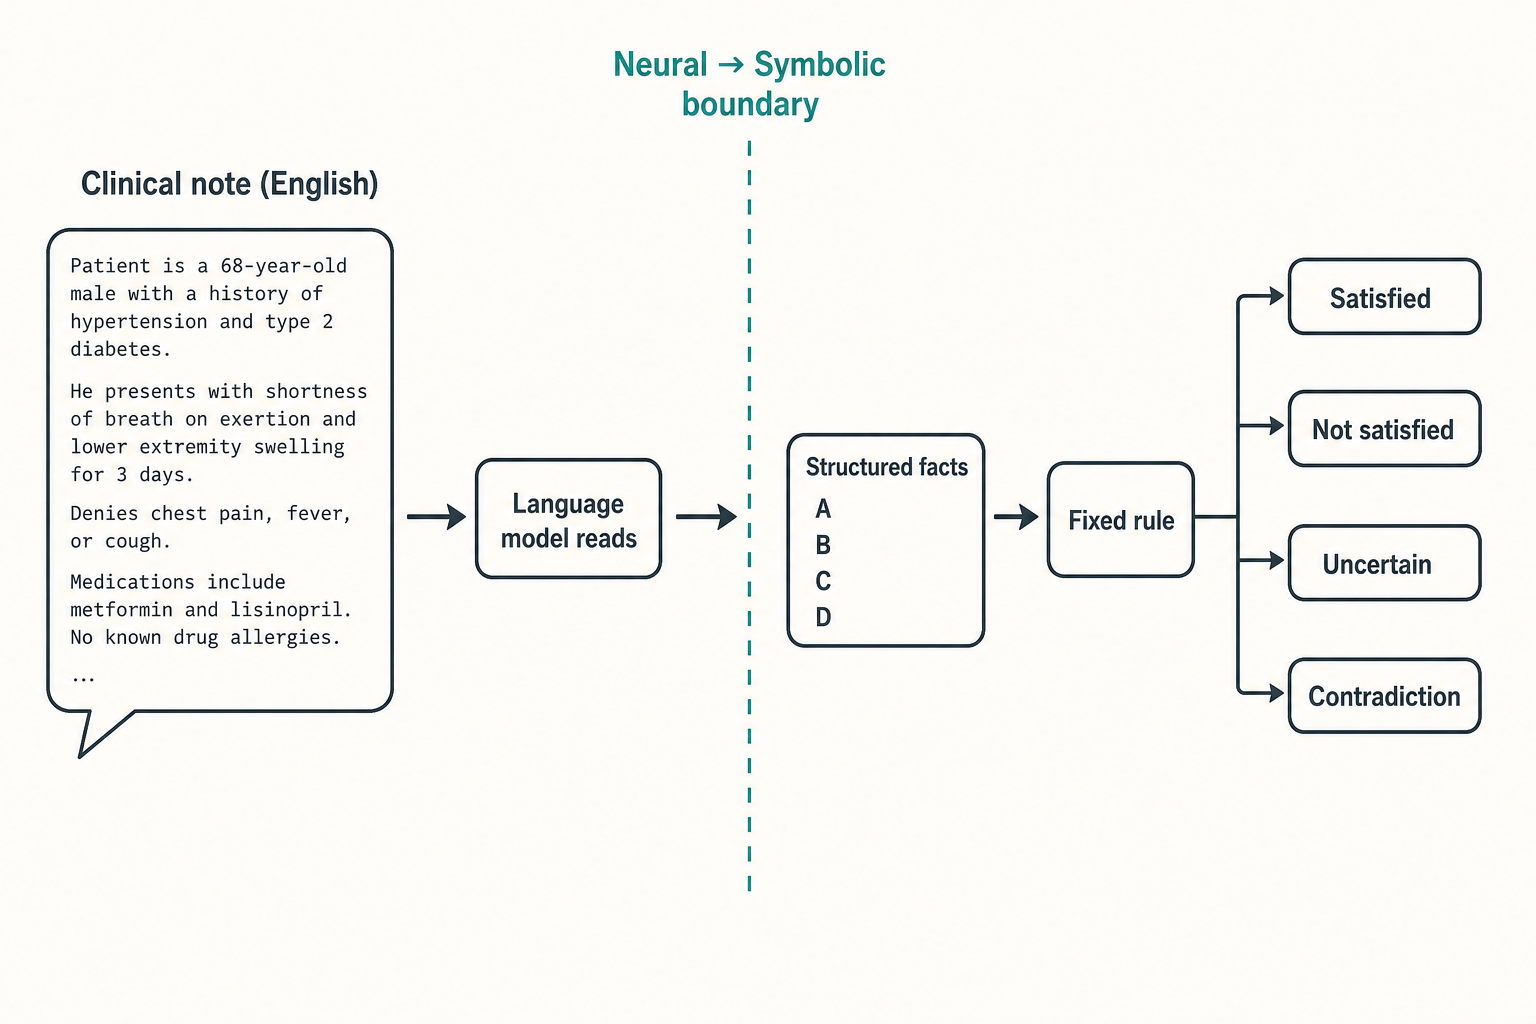
\includegraphics[width=0.92\textwidth]{figures/nesy-boundary-simple.png}
\captionof{figure}{A language model fills an extract. A fixed rule --- not the model --- issues the label.}
\end{center}

This mapping pass never rewrote that rule. We only edited the \textbf{extract} (Translate), then ran the same \texttt{ground()} and the same rule.

\section{What we set out to do}

Ambitious sentence (later thesis, not this freeze): automatically correct every failure mode in a large language model.

Smaller question we actually ran:

\begin{quote}
When Dual is wrong on ``did first-line therapy fail?'', can we \emph{group} those mistakes and \emph{patch the extract} without breaking notes that were already right --- and later \emph{choose} a patch?
\end{quote}

\textbf{Answer we froze:} grouping and patching --- partial yes. Choosing among independent editors --- no. Generic auto-correct --- no.

\section{The Dual question}

Synthetic notes (not real patients). Four facts plus a conflict flag:

\begin{center}
\begin{tabular}{@{}ll@{}}
\toprule
Atom & Plain meaning \\
\midrule
A & A first-line therapy is identified \\
B & It was actually given, not only planned \\
C & Something that counts as failure happened \\
D & That failure is \emph{of} first-line \\
X & Two claims cannot both be true \\
\bottomrule
\end{tabular}
\end{center}

Rule (unchanged): if X then CONTRADICTION; else if any of A--D is false then NOT\_SATISFIED; else if any is unknown then UNCERTAIN; else SATISFIED.

\section{What we built}

Nested Translate patches \textbf{none $\rightarrow$ G3 $\rightarrow$ G4 $\rightarrow$ G6 $\rightarrow$ G7 $\rightarrow$ G8 $\rightarrow$ G9}.
Deeper includes earlier. That is one class of edit, not six products.

On 108 Dual-fill notes: raw Dual-wrong 30; after G9 leftover 6. P-neg leak 0 after G3. Design P-bind 7/7 match after G9.

\section{Walk the GUI}

Start the viewer:

\begin{verbatim}
cd ~/staging/cxr-evidence-grounding-lab
./scripts/run_map_viewer.sh
\end{verbatim}

Open \url{http://127.0.0.1:8263/}. Read the yellow banner (mapping, not selection).

\begin{enumerate}
  \item Click \textbf{T1}. Gold SATISFIED. Every row already matches. This note needed no patch.
  \item Click \textbf{I2}. Raw extract is NOT\_SATISFIED (\texttt{admin=planned}). G9 flips planned $\rightarrow$ given. SATISFIED.
  \item Click \textbf{C4}. Gold CONTRADICTION. G4 is the first match; G8 is a deeper signature.
  \item Click \textbf{T2} (or filter ``Still miss after G9''). Too early for a failure event. Leave it unrepaired.
\end{enumerate}

Curriculum reading UI: \url{http://127.0.0.1:8264/}. Frozen locator \texttt{:8260} is a different product --- do not expand it here.

\section{What we are (and are not) claiming}

\begin{itemize}
  \item \textbf{Are:} Dual-shaped extract failures can be grouped; some can be patched on the Translate side with measured collateral.
  \item \textbf{Are not:} a generic LLM auto-corrector; locator-chosen Encode vs Compute vs Translate; six independent editors; leftover-6 as unfinished homework.
\end{itemize}

\section{Where to go next}

\begin{center}
\begin{tabular}{@{}ll@{}}
\toprule
\textbf{Want\ldots} & \textbf{Open\ldots} \\
\midrule
Click notes & \url{http://127.0.0.1:8263/} \\
Study modules & \url{http://127.0.0.1:8264/} \\
Every number & \texttt{notes/mapping-notes.pdf} \\
Runnable Python & \texttt{notes/mapping-code-walkthrough.pdf} \\
Course PDF & \texttt{notes/CXR-Mapping-Curriculum.pdf} \\
Older N2S notebook & \texttt{notes/progress-notes.pdf} \\
Older simple guide & \texttt{notes/progress-notes-simple.pdf} \\
Design doc & \texttt{docs/TRACKB-FAILURE-INTERVENTION-MAP.md} \\
\bottomrule
\end{tabular}
\end{center}

\vspace{1em}
\begin{center}
\color{muted}\small
Rebuild: \texttt{./build-mapping-pdfs.sh} from the \texttt{notes/} directory.
\end{center}

\end{document}
